\section{Imperative to Streaming Transformation}
\label{sec:control}

%In a na\"ive approach, we can map each controller in the hierarchy into a VB (\Cref{fig:centralctrl}).
%This strategy suffers from expensive network round-trip delays between the parent and child controllers.
%If the parent controller is an unrolled loop, the parent needs to synchronize with all child controllers, which creates an undesired communication hot spot.
%\Cref{fig:centralctrl}(a) shows an example where synchronization {\em just} between parent and child controllers can produce an incorrect result due to unpredictable network latency.

%The alternative approach explores a different way to execute the expected control schedule correctly. 
%The minimum required synchronization to produce the correct result is to ensure that the computations access the intermediate results in a consistent matter as if the control schedule is strictly enforced. 
%This can be achieved via p2p synchronizations \emph{only} between computations that access a particular shared memory.
%The execution order of computations that access different memories does not need to be enforced, as they do not impact the program outcome.
%Therefore, as long as the compututation is executed with the expected number of iterations and the memories are updated consistently, there is no need for any extra synchronization.
%Next, we walk through how \name{} achieves this in more concrete detail.

\subsection{Loop Division (Ready)}
Between the front-end and back-end abstraction of \name, an obvious gap between the two abstractions is that the front-end imperative language can contain arbitrarily nested control hierarchy, whereas
the hardware compute engine can only execute perfectly nested loops.
To address this issue, we introduce a new type of loop transformation---loop division---for streaming reconfigurable
accelerators.
Similar to loop fission, loop division breaks a single loop into multiple loops.
The difference is that loop fission generates a sequence of sequentially executed loops, whereas
loop division generates loops executing \emph{concurrently}.
Additionally, loop fission materializes the intermediate results across fissioned loops into arrays,
while loop division use queue to communicate across loops.
Each loop generated from loop division can only execute if all of their input queues are not empty.
\Cref{fig:loopexp1} gives an example of a loop fusion vs. loop division.

\begin{figure*}
\centering
\begin{subfigure}[b]{0.28\textwidth}
\inputminted{python}{code/loopexp1.py}
\caption{Input program}
\end{subfigure}
\hfill
\begin{subfigure}[b]{0.31\textwidth}
\inputminted{python}{code/loopexp1fission.py}
\caption{Loop Fission}
\end{subfigure}
\hfill
\begin{subfigure}[b]{0.32\textwidth}
\inputminted{python}{code/loopexp1division.py}
\caption{Loop Division}
\end{subfigure}
\caption[Example of loop fission vs. loop division]{
  (b) and (c) shows the output of loop fission and loop division of the input program (a), respectively.
  In (b), the first loop is executed entirely before executing the second loop. The intermediate
  result \texttt{tmp} is materialized into an array with the same size as the loop range.
  In (b), the two loops can execute concurrently. The intermediate result is materialized into a
  queue. For each iteration, a loop can execute only if all of its queues are non-empty.
  The second loop can execute as soon as \texttt{tmp} receives the first element.
}
\label{fig:loopexp1}
\end{figure*}

When executing loop division on a single-threaded CPU, the CPU must context switching between the
concurrent loops
and executing the one with cleared input dependencies.
Like loop fission, loop division is likely worsening the performance on a processor architecture, as
the worst-case memory footprint of the intermediate result \texttt{tmp} increases from $O(1)$ to $O(N)$.
On RDAs, the divided loops are executing
concurrently in a streaming pipelined fashion. The size of the \texttt{tmp} can be limit to a small fixed
size, efficiently implemented with a hardware FIFO. 
Although loop transformations are generally optimizations on CPUs,
loop division is a required transformation to converts an infeasible program to a feasible one for Plasticine.

Loop fission is not always safe, as it may alter the execution order of the program.
Loop division, on the other hand, does not change the underlying data-dependency and is always safe.
To achieve this, loop division needs to introduce additional dummy data dependencies across divided
loops to enforce the correct execution order.
\Cref{fig:loopexp2} gives an example of an invalid loop fission and a correct loop division.
\Cref{fig:sync} gives more detail on how \name automatically generates the dummy data-dependencies.

\begin{figure*}
\centering
\begin{subfigure}[b]{0.28\textwidth}
\inputminted{python}{code/loopexp2.py}
\caption{Input program}
\end{subfigure}
\hfill
\begin{subfigure}[b]{0.32\textwidth}
\inputminted{python}{code/loopexp2fission.py}
\caption{Invalid Loop Fission}
\end{subfigure}
\hfill
\begin{subfigure}[b]{0.31\textwidth}
\inputminted{python}{code/loopexp2division.py}
\caption{Loop Division}
\end{subfigure}
\caption[Example of an illegal loop fission and a legal loop division]{
Example of an illegal loop fission and a legal loop division
}
\label{fig:loopexp2}
\end{figure*}

\subsection{Virtual Context Allocation (Ready)} 

\begin{figure*}
\centering
\begin{subfigure}[b]{0.4\textwidth}
\inputminted{python}{code/spatialeg.py}
\caption{Pseudo input example}
\label{fig:contexteg}
\inputminted{python}{code/contextalloc.py}
%\missingfigure[figwidth=1\textwidth]{Spatial IR}
\caption{Context allocation}
\end{subfigure}
\hfill
\begin{subfigure}[b]{0.5\textwidth}
\inputminted{python}{code/contextsplit.py}
\caption{Request and response division}
\end{subfigure} \\
\vspace{0.2cm}
\begin{subfigure}[b]{0.23\textwidth}
%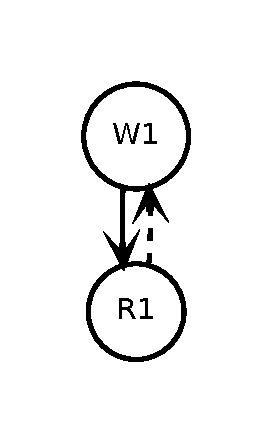
\includegraphics[width=1\textwidth]{figs/dep.pdf}
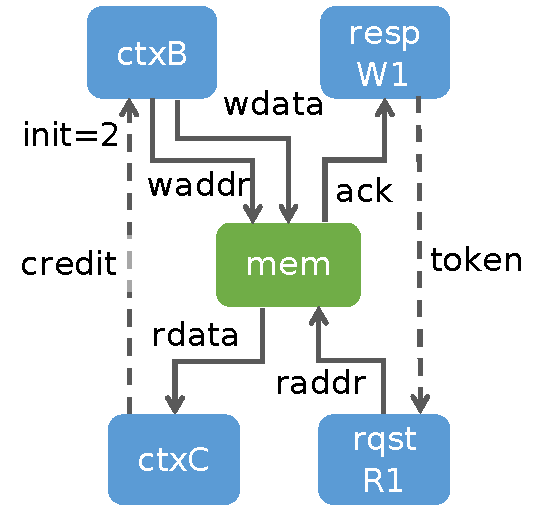
\includegraphics[width=1\textwidth]{figs/ctxdag.pdf}
\caption{Context Graph}
\end{subfigure}
\begin{subfigure}[b]{0.76\textwidth}
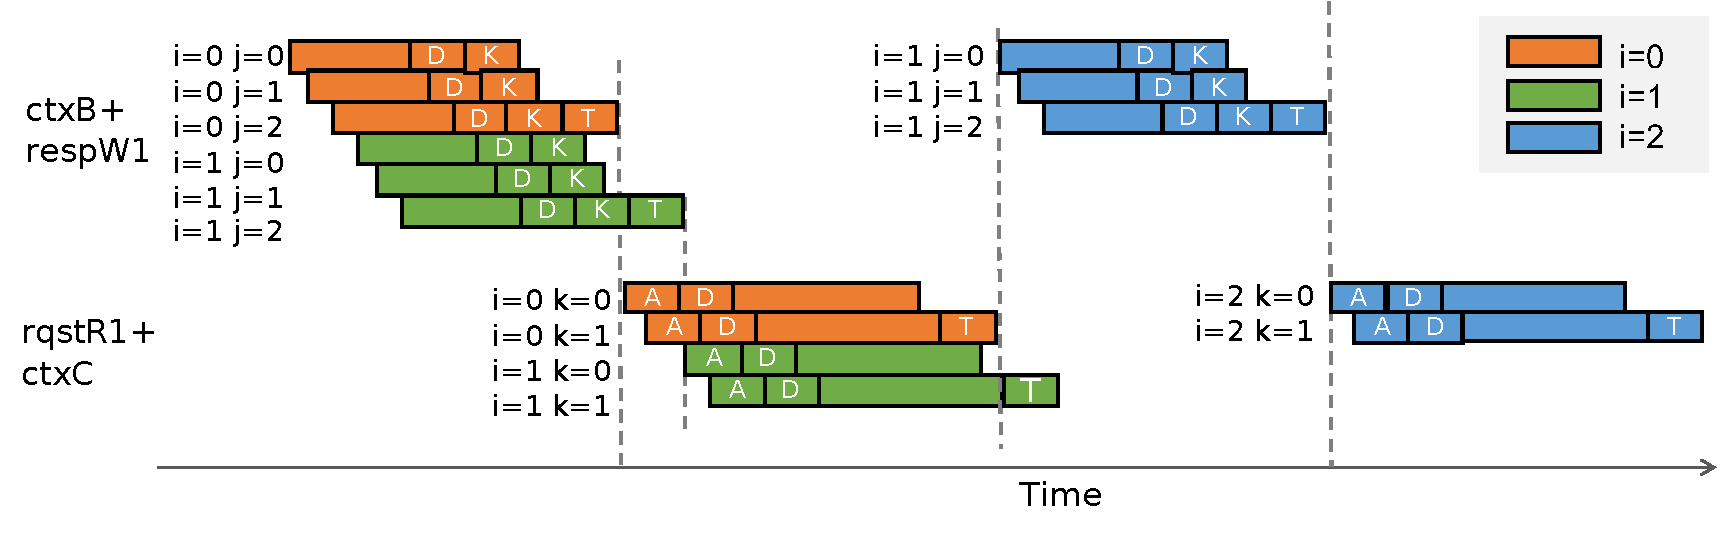
\includegraphics[width=1\textwidth]{figs/plasticinetiming.pdf}
\caption{Timing on Plasticine}
\end{subfigure}
\caption[Context allocation]{
  Lowering example.
  %Same example as \Cref{fig:spatialegpar} without outer loop
  %unrolling factor equals to 1.
  %(a) has two basic blocks within the inner most controllers \texttt{B} and \texttt{C}.
  \name allocates one context per basic block for \texttt{B} and \texttt{C}, shown in (b). Outer controller \texttt{A} is
  duplicated in both \texttt{ctxB} and \texttt{ctxC}.
  (c) \name seperates out requestion generator \texttt{rqstR1} from \texttt{ctxB} for \texttt{R1} 
  and response receiver from \texttt{ctxC} \texttt{respW1} for \texttt{W1}.
  The resulting dataflow graph is shown in (d). 
  To enforce the forward data-dependency between \texttt{W1} and \texttt{R1}, 
  \name allocates a forward token between \texttt{W1}'s response receiver \texttt{respW1} and
  \texttt{R1}'s request generator \texttt{rqstR1};
  to enforce the loop-carried WAR dependency between \texttt{R1} and \texttt{W1}, \name allocates a
  backward token (\texttt{credit}) between \texttt{R1}'s response receiver \texttt{ctxC} and 
  \texttt{W1}'s request generator \texttt{ctxB}. 
  The backward credit is initialized with two elements because \texttt{mem} is double-buffered.
  On the writer side, a forward \texttt{token} is a
  produced and a backward \texttt{credit} is consumed every \texttt{B} iterations; on the reader
  side, a forward \texttt{token} is consumed and a backward credit is produced every \texttt{C}
  iterations. The resulting timing of the execution is shown in (e).
}
\label{fig:contextalloc}
\end{figure*}

As a start, \name allocates one virtual memory to hold each on-chip data structure, and 
one context to execute each basic block within the innermost controllers. 
A basic block maps naturally to a context, as instructions within a basic block are control-free. 
Next, \name makes a copy of all controllers enclosing the basic block in the corresponding context;
these controllers are later converted to counters and control configurations supported by the
hardware. 
Effectively, \name performs loop division such that all basic blocks are perfectly nested.
\Cref{fig:contextalloc} shows an example of the context allocation. 
With these controllers, contexts can repeat execution for expected number iterations. However,
data-structures written and read by different contexts are accessed in random order.
The insight is that \emph{as long as all contexts accessing a shared memory with expected program order, the final result is identical to a sequentially executed program}.
Unlike traditional out-of-order execution, where hardware and compiler look for independent instructions to
execute concurrently, \name starts with executing \emph{all} basic blocks in a program in \emph{concurrent} contexts.
Next, \name introduces synchronizations to maintain consistent access order as expected by the program \emph{only} among contexts accessing a shared memory. 
This way, \name introduces minimum p2p synchronizations among small groups of contexts; contexts
accessing different memories are naturally parallelized without impacting the final output.

\subsection{Control Allocation (WIP)} 
\label{sec:sync}
Starting with all contexts execute in parallel, \name introduces \term{control token}s across contexts
to serialize their execution order based on the program order.
This control token is no different from a regular data-dependency and can be viewed as 
an access grant to the shared memory across contexts. 
By controlling {\em where}, {\em how}, and {\em when} to pass the token, \name is able to maintain a consistent update ordering between the pipelined and parallelized contexts that access the shared memory.

We refer to a memory access appeared in the input IR as a \emph{declared access}, as supposed to
memory accesses executed at runtime.
\texttt{W1} and \texttt{R1} are examples of two declared accesses in \Cref{fig:contexteg}
In the rest of this section, we will walk through how \name allocates control tokens
to maintain sequential consistency on Plasticine.

\begin{table*}
  \centering
\begin{tabular}{lccc}
  \toprule
 Data structure & Memory type \\ \midrule
  array (fit on-chip) & SRAM \\
  array (not fit on-chip) & DRAM \\
  scalar variable & register \\
  queue & FIFO \\
 \bottomrule
\end{tabular}
\caption[Mapping between data-structure to hardware memories]{
  Mapping between user declared data-structure to underlying hardware memories. 
  Programmers explicitly specify the desired hardware type inside Spatial. 
  In other languages, this table specifies a mapping between software data-structures 
  and hardware memory types on Plasticine.
}
\label{tab:memtype}
\end{table*}

\paragraph{Where.}
During control allocation, \name examines all declared accesses of a memory and checks for dependency across these accesses.
\name only allocate resource to synchronize two contexts if they contain declared accesses that can potentially interfere.
Whether two declared accesses interfere depends on 
\begin{outline}
  \1 the type of accesses (read vs. write)
  \1 the type of the memory (e.g. SRAM, DRAM)
  \1 and location of the declared accesses in the control hierarchy.
\end{outline}

\begin{table*}
  \centering
\begin{tabular}{lcccc}
  \toprule
  Memory type             & DRAM   & SRAM   & FIFO   & Register \\ \midrule
  read-after-read (RAR)   & \xmark & \cmark & \cmark & \cmark \\
  read-after-write (RAW)  & \cmark & \cmark & \cmark & \cmark \\
  write-after-read (WAR)  & \cmark & \cmark & \cmark & \cmark \\
  write-after-write (WAW) & \cmark & \cmark & \cmark & \cmark \\
 \bottomrule
\end{tabular}
\caption[Interferance Table]{
  Interference table for whether two accesses interfere for each memory type.
}
\label{tab:interferetab}
\end{table*}

\Cref{tab:memtype} lists hardware memories available on reconfigurable architectures and software data-structures providing similar program semantics.
The type of the memory matters because they have different programming interface on the hardware.
For instance, two DRAM read accesses do not interfere because the DRAM interface permits
multiple concurrent access streams through multiple DAGs\footnote{All DAGs can access the full DRAM
address space}. 
%\gist{mension port virtualization}
Therefore, from the programmer's perspective, users do not need
to serialize the two contexts reading the same DRAM address. 
SRAMs, on the other hand, have a single read and write port. Programmers must guarantee that a PMU receives read requests from a single context
at any point in time for correctness.
\Cref{tab:interferetab} shows the interference relation between different types of memory across
accesses.

\begin{figure*}
\centering

\begin{subfigure}[b]{0.5\textwidth}
\inputminted{python}{code/dep1.py}
\caption{Pseudo example}
\end{subfigure}
\begin{subfigure}[b]{0.3\textwidth}
  \centering
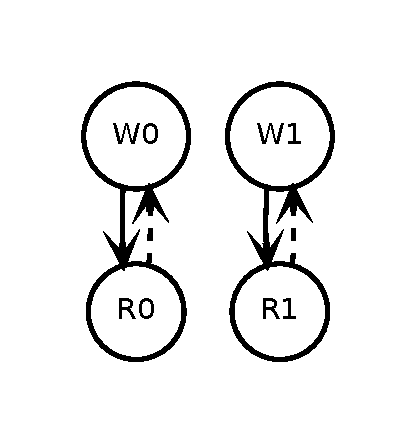
\includegraphics[width=0.8\textwidth]{figs/dep1.pdf}
\caption{Dependency Graph}
\end{subfigure}
\\
\begin{subfigure}[b]{0.5\textwidth}
\inputminted{python}{code/dep3.py}
\caption{Pseudo example}
\end{subfigure}
\begin{subfigure}[b]{0.3\textwidth}
  \centering
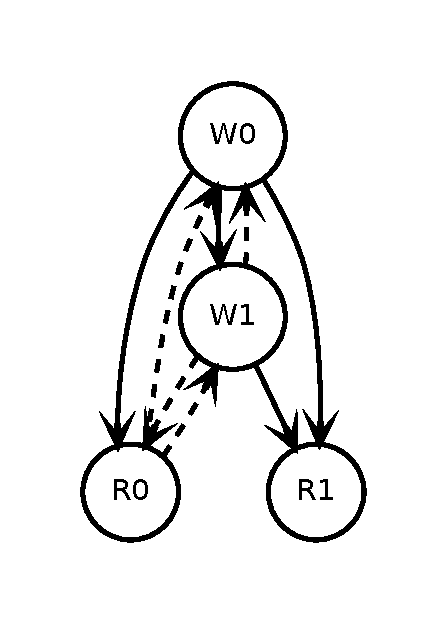
\includegraphics[width=0.8\textwidth]{figs/dep3.pdf}
\caption{Dependency Graph}
\end{subfigure}

\caption[Dep Graph]{
  Dep Graph (WIP)
}
\label{fig:depexp}
\end{figure*}

For every declared access, \name{} checks on other accesses appeared earlier in the program order
for a possible forward dependency, and later in the program order for a possible loop-carried dependency (LCD). 
In the example in \Cref{fig:contexteg}, there is a forward data dependency between \texttt{W1} and
\texttt{R1}, and a write-after-read LCD between \texttt{R1} and \texttt{W1}. 
\name builds a dependency graph between declared accesses for each memory.
\Cref{fig:depexp} gives more examples of how \name
determines dependencies based on where these accesses are declared in the control hierarchy.

Enforcing all dependencies in the dependency graph may not be necessary, as enforcing a subset of
dependencies can be sufficient to enforce the order of the whole graph.
Therefore, \name performs a transitive reduction (TR) on the graph to keep the minimum number of dependency edges that preserve the same ordering \cite{tr}.
Since TR on a cyclic graph is NP-hard, \name perform TRs on the forward and backward LCD graphs, separately.
Notice, dependencies between accesses touching different buffers of a multi-buffered memory is less rigid than accesses touching the same buffer.
Therefore, we can only remove an edge if all dependencies on the equivalent path have a stronger or equivalent dependency strength than the strength of the removed edge.

%Two declared accesses A and B have no dependency if their least-common ancestor (LCA) controller executes only one of the children at anytime (from a branch), or all children in parallel (from an unrolled loop).
%The LCD exists between B to A, if B occurs later in the program order, and A and B are surrounded by a loop.
%To detect LCD, \name checks if a loop exists among two accesses' LCA controller and LCA's ancestor controllers.

\begin{figure*}
\centering
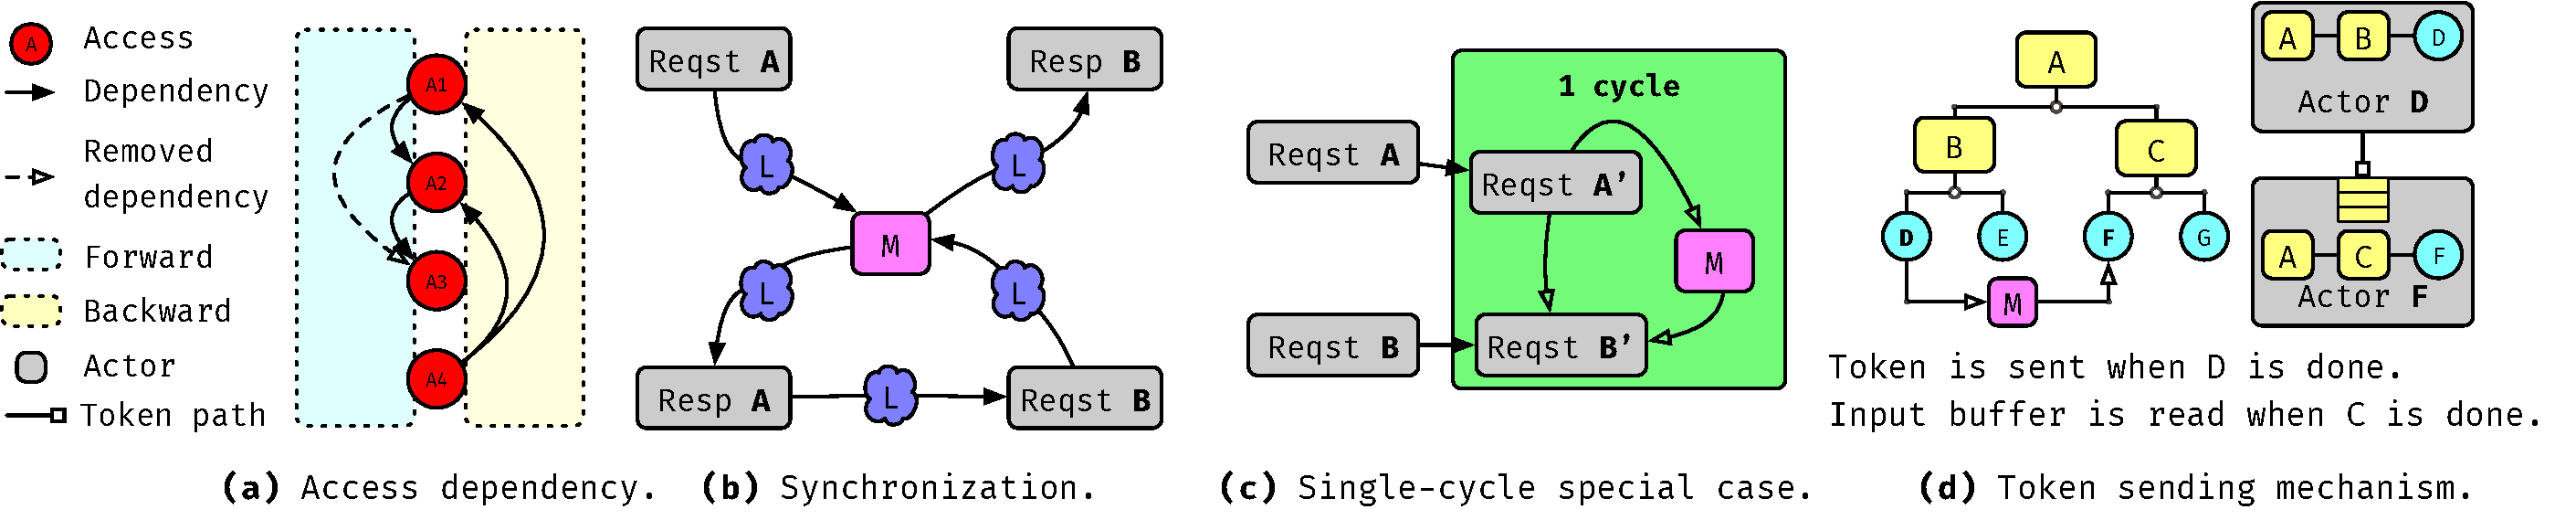
\includegraphics[width=1.0\textwidth]{figs/synch_mech.pdf}
\caption{
    (a) Access dependency graph.
    (b) Synchronization of two accesses on the same memory.
    (c) Single-cycle special case.
    (d) Actors uses local states of controller hierarchy to determine when to send a token.
}\label{fig:depgraph}\label{fig:token}\label{fig:tokentrick}\label{fig:tokenwhen}
\end{figure*}
%\ms{repeated caption, rather give a single caption.}

\paragraph{How.} 
%For each intermediate memory, \name{} builds a dependency graph for all its declared accesses (\Cref{fig:depgraph}(a)).
%Enforcing all dependencies in this graph may not be necessary as dependencies between $A_1$ and $A_2$, and $A_2$ and $A_3$ already capture the dependency between $A_1$ and $A_3$.

To eliminate the round-trip overhead between the memory and the computation, 
\name{} duplicates the local states and expressions required to generate the requests in a separate context as the one that handles the responses.
For write accesses, the memory provides an acknowledgment for each request received, used by \name for synchronization.
The request context generates requests asynchronously as soon as its data-dependencies are cleared, pushing all requests to memory until back-pressured.
To order a declared access A before a declared access B
\name creates a dummy dependency between the context that accumulates the response of access A ($resp_A$) and the context that generates requests for access B ($reqst_B$) (\Cref{fig:token}(b)).
To enforce LCD from access B to access A, \name introduces a token from $resp_B$ to $reqst_A$, and initializes the token buffer (input buffer receiving the token) with one element to enable the execution of the first iteration.
If the LCD is on a multi-buffered memory, the LCD token is initialized with the buffer depth number of elements to enable A for multiple iterations before blocked by access B.

These are general schemes we use on any type of memory (including DRAM and on-chip memories) with unpredictable access latency.

\paragraph{When.}
\name{} configures the contexts to generate the token using their local states at runtime.
For FIFOs, the token is generated and consumed every cycle when the producer and receiver contexts are active.
For register, SRAM, and DRAM, the program order expects that the producer and consumer write and inspect the memory once per iteration of their LCA controller, respectively.
Since the producer and receiver both have their outer controllers duplicated in their local state, they have independent views for one iteration of the LCA controller, which is when the controller in their ancestors (that is the immediate child of the LCA controller) is completed (\Cref{fig:tokenwhen}(d)).
The {\em done} signals of these controllers are used to produce and consume the token in contexts, independently.

\paragraph{Specialization for dense on-chip array}
For a memory with guaranteed {\em single-cycle} access latency, such as registers and statically banked SRAMs that are guaranteed conflict-free, we can simplify the necessary synchronization (\Cref{fig:tokentrick}(c)).
Instead of synchronizing between $resp_A$ and $reqst_B$, we allocate two stateless contexts $reqst_A'$ and $reqst_B'$ within {\emph the same} VB as the accessed memory that forwards requests from $reqst_A$ and $reqst_B$, respectively.
Next, we forward the token going from $reqst_A$ to $reqst_B$ to go through $reqst_A'$ to $reqst_B'$ instead, and configure the token buffer in $reqst_B'$ with the depth of one for serialized schedule and depth of M for multi-buffered schedule. 
We no longer need to insert the LCD token, as the stiff back pressure from the token buffer in $reqst_B'$ will enforce the expected behavior.
This optimization only works if the sender and receiver of the token buffer are physically in a single VB where the memory is located.
In this way, when $reqst_B'$ observes $reqst_A'$s token, $reqst_B'$ is guaranteed to observe the memory update from $reqst_A'$ because the memory also has single-cycle access latency.

\paragraph{Specialization for non-indexable memory}
We perform another specialization on non-indexable memories (registers or FIFOs), whose all accesses have no explicit read enables.
Instead of treating them as shared memories, \name{} duplicates and maps them to local input buffers in all receivers, no longer requiring tokens.
The sender actor pushes to the network when the token is supposed to be sent, and the receiver dequeues one element from the input buffer when the token is supposed to be consumed.
This dramatically reduces the synchronization complexity of non-indexable memory in the common case.

\subsection{Data-Dependent Control Flow (Ready)}
Using the synchronization discussed in \Cref{sec:sync}, \name can support control constructs that 
typically are not supported on dataflow accelerators, such as branches and while loops.
Most dataflow accelerators do not support control divergence. SIMT architectures, like GPUs,
implement branches with predications and pay the latency penalty of both branch cases.
To enable these flexible control, the control path of the architecture must permit data dependencies.
\Cref{fig:controlarch} details the required changes in the control path to support these features.

\paragraph{Dynamic Loop Range}
\Cref{fig:dynrange} shows an example of loops with data-dependent ranges. 
\name uses a context to compute the loop bounds, which are treated as input dependency to the context 
that maps the loop body.
\begin{figure*}
\centering
\begin{subfigure}[b]{0.4\textwidth}
\inputminted{python}{code/dynrange.py}
\caption{Input program}
\end{subfigure}
\hfill
\begin{subfigure}[b]{0.5\textwidth}
\inputminted{python}{code/dynrangectx.py}
\caption{Context graph}
\end{subfigure}
\caption[Example of dynamic loop range]{
  (a) shows an example program with dynamic loop range. 
  Expressions to generate the loop bounds belongs to a basic block that gets mapped to \texttt{ctx1}.
  \name maps the loop bound as a data-dependnecy to context that maps the inner loop context, and
  configures dequeue signal of \texttt{bound} stream to counter \texttt{B.done}.
}
\label{fig:dynrange}
\end{figure*}

\begin{figure*}
\centering
  \vspace{-1cm}
\begin{subfigure}[b]{0.45\textwidth}
\inputminted{python}{code/branch.py}
\caption{Input program}
  \vspace{0.2cm}
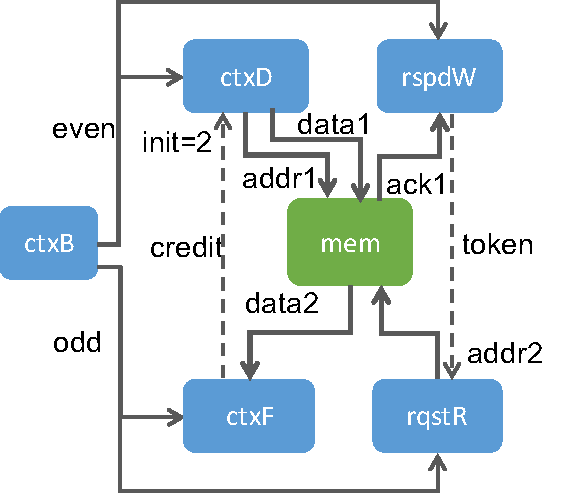
\includegraphics[width=0.8\textwidth]{figs/branchctx.pdf}
\caption{Dataflow graph}
\end{subfigure}
\hfill
\begin{subfigure}[b]{0.48\textwidth}
\inputminted{python}{code/branchctx.py}
\caption{Context configuration}
\end{subfigure}
\\
  \vspace{0.2cm}
\begin{subfigure}[b]{\textwidth}
  \centering
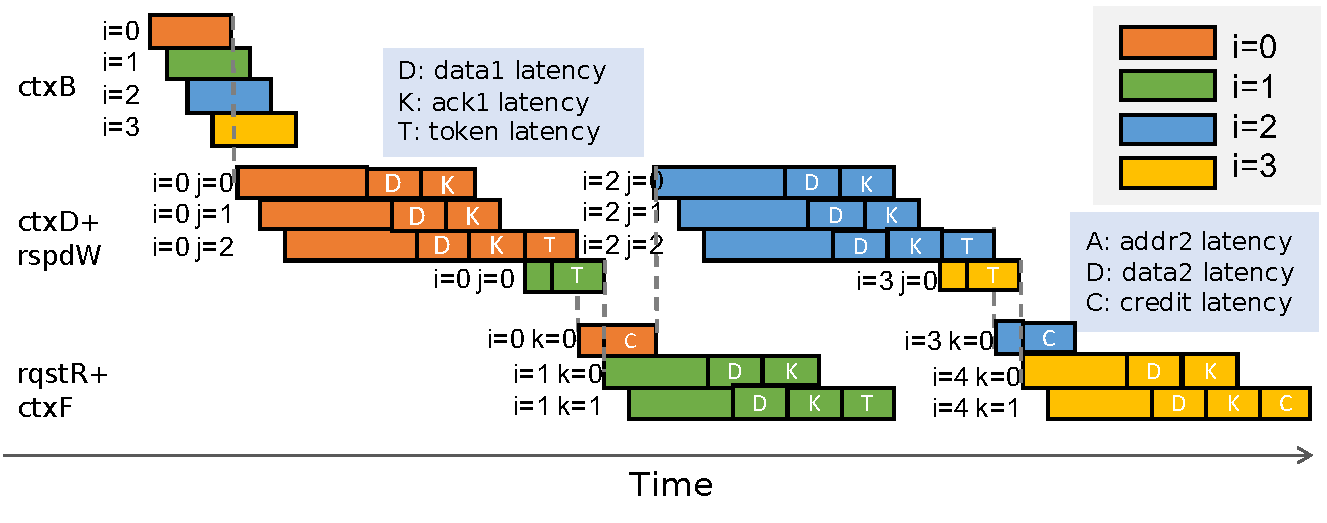
\includegraphics[width=0.8\textwidth]{figs/branchtiming.pdf}
\caption{Timing}
\end{subfigure}
\caption[Branching example]{
  An example program with a branch. 
  (d) shows the timing of execution with $A=4$, $D=3$, and $F=2$.
}
\label{fig:branch} 
\end{figure*}

\paragraph{Branch Condition}
\name supports both predictions and actual branches.
Branches within the innermost loops are implemented with predications so that the loop can still be
vectorized across SIMD lanes.
This is very similar to a SIMT architecture, where all lanes execute the \emph{if} clause followed by the \emph{else} clause, masking off the memory access for the disabled lanes.
The total number of stages required is the total operations in both the \emph{if} and the \emph{else} clauses.

For an actual branch in an outer loop,
the branch condition is treated as a data-dependent enable signal for controllers under the branch clauses.
If the controller is disabled, its \emph{done} signal raises to high immediately.
Output tokens depending on the {\em done} signal will be immediately sent out.
This way, the controller under a branch condition does not need to execute if the outer branch
evaluates to false.

\Cref{fig:branch} shows an example with a branch statement.
The input program in (a) writes and reads the memory \emph{mem} on even and odd cycles of
the outer loop \emph{A}, respectively. 
\name maps the three basic blocks in the program in three
contexts, \emph{ctxB}, \emph{ctxD}, and \emph{ctxF}, as shown in (b) and (c). 
For the read and write accesses, \name
allocates a context \emph{respW} to accumulate write acknowledgments and a context \emph{rqstR} 
to generate read requests. 
\emph{ctxB} generates the branch conditions for both the \emph{if} and the \emph{else} clauses.
The conditions are sent as data dependencies to contexts mapping the basic blocks under the branch conditions.

\Cref{fig:branch} (d) shows the timing of execution.
As \emph{ctxB} has no dependencies, \emph{ctxB} computes the conditions for all iterations of
\emph{A} in
pipelined fashion and broadcasts the conditions to the receiver contexts.
The \emph{if} contexts (\emph{ctxD}+\emph{rspdW}) receives a \texttt{true} condition for the first
iteration of \emph{A} ($A_0$), 
executing all iterations of D, and passes a token to the \emph{else} (\emph{rqstR}+\emph{ctxF}) contexts.
Because \emph{mem} is double-buffered, the credit is initialized with two elements in the
receiver's input buffer, enabling the \emph{if} contexts to execute two iterations of outer loop
\emph{A} before
waiting for the \emph{else} contexts. For the second iteration of loop \emph{A} ($A_1$), the \emph{if} contexts
receives a \texttt{false} condition for branch \emph{C}.
Therefore, the enclosing loop controller \emph{D}'s \emph{done} signal is immediately high, sending the
token to \emph{rqstR} context right away.
On the other side, the $A_0$ of the \emph{else} contexts is blocked by the token from
the \emph{if} contexts. 
As soon as the token arrives, the \emph{else} contexts send out the credit immediately,
Next, the \emph{else} contexts check for the second token, 
and executes loop \emph{F} for $A_1$.

Both the \emph{if} and the \emph{else} contexts only execute if their enclosed branch clauses are
evaluated to be true. More interestingly, \Cref{fig:branch} (d) shows a overlapping execution of the
\emph{if} and \emph{else} clauses across iterations of A. 
The hardware for both \emph{if} and \emph{else} clauses are active almost all time.
If the latency of loop \emph{D} and \emph{F} are both $L$, 
the total runtime for $N$ iterations of loop \emph{A} would be on the order of $\frac{N}{2}L+L$
on Plasticine, assuming L and N are large.
\emph{This is almost twice as fast as a traditional coarse-grained pipelining with hierarchical FMS
schedulers}, like Spatial's FPGA back-end, whose runtime is $NL+L$.

\paragraph{Do While Loops}

\begin{figure*}
\centering
  \vspace{-1cm}
\begin{subfigure}[b]{0.45\textwidth}
\inputminted{python}{code/dowhile.py}
\caption{Input program}
  \vspace{0.2cm}
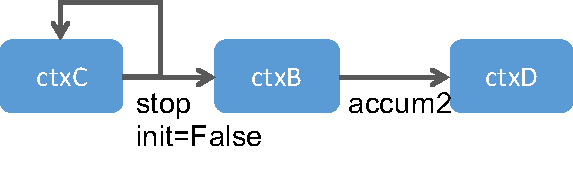
\includegraphics[width=0.8\textwidth]{figs/dowhile.pdf}
\caption{Dataflow graph}
\end{subfigure}
\hfill
\begin{subfigure}[b]{0.48\textwidth}
\inputminted{python}{code/dowhilectx.py}
\caption{Context configuration}
\end{subfigure}
\\
  \vspace{0.2cm}
\begin{subfigure}[b]{\textwidth}
  \centering
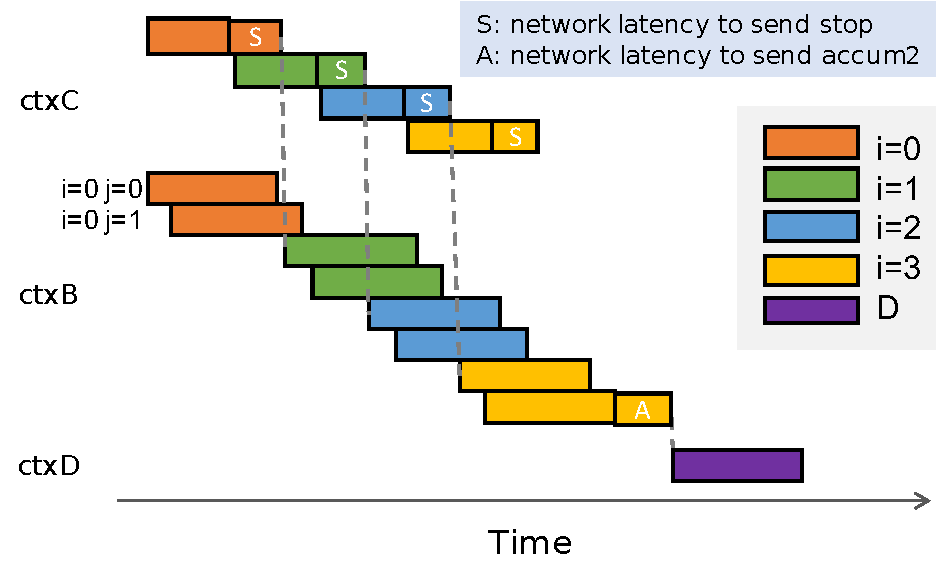
\includegraphics[width=0.6\textwidth]{figs/dowhiletiming.pdf}
\caption{Timing}
\end{subfigure}
\caption[Do while example]{
  An example program for do while loop. 
  Loop \emph{A} in (a) is a loop running forever, with a conditional \emph{stop} variable.
  The break statements in (c) corresponds to configuring the stop signal of the enclosing controller \emph{A}
  to the output of the stop input buffer. The stop buffer is dequeued every cycle controller \emph{A} is active.
}
\label{fig:dowhile} 
\end{figure*}

The \emph{do while} construct is very useful to express iterative convergence algorithms or handle external
data stream with a last-bit signal that terminates the execution.
A \emph{do while} loop works very similarly to a loop with dynamic range, except the loop has a very long
initialization interval. The earliest starting time for the second iteration of the loop is when the while condition is resolved.
The while condition is a data-dependency to all contexts mapping the basic blocks enclosed by the while loop.
%This while condition is a loop carried dependency, assuming the first value is produced after the first
%iteration.
There is a loop-carried dependency between the producer of the condition within the while loop body
and the loop controller that consumes a value of condition every iteration.
\Cref{fig:dowhile} shows an example with a do-while loop.

%The break statement in (a) translates to a \emph{stop} register associated with the controller of loop
%\emph{A}. 
Loop \emph{A} reads and block \emph{C} writes a value of stop for every iteration of loop
\emph{A}.
\Cref{fig:dowhile} (b) shows the dataflow graph, mapping each basic block to a context.
\emph{ctxC} computes the stop condition, which is used by both \emph{ctxC} and \emph{ctxB}.
There is a loop-carried dependency between the reader of \emph{stop} from loop \emph{A} and the
writer of stop from block \emph{C}. Therefore, the stop streams in (c) are initialized with 
\texttt{False} to enable the execution of the first iteration.
The \emph{accum} variable in (a) has two readers in block \emph{B} and block \emph{D}; one has a
loop-carried dependency with the writer (line 9) and the other has a forward data-dependency (line
11). 
Therefore, the variable is mapped to two copies of \emph{accum}, one for each reader. 
Because the accumulate operation is a single operation ADD, the accumulator gets optimized to the special
accumulate pipeline register \emph{accum1}, 
Without this optimization, \emph{accum1} would be another \texttt{ScalarStream} with an initial
element 0.
The other \emph{accum} becomes a scalar stream \emph{accum2}, written by \emph{ctxB} when loop \emph{A}
is done.
(d) shows the timing of execution. As we can see, the initialization interval across iterations of
A in the steady-state is bounded by the latency to evaluate \emph{stop}, which is the number of
operations in stop expression rounded up to a multiple of 6 stages because the data must
propagate to the end of each SIMD pipeline.

\subsection{Virtual Unit Allocation (Ready)}
After all contexts and shared memory are allocated and synchronized, 
\name moves the remaining floating contexts into their own VUs, indicating the boundary of the physical units.
Certain contexts mentioned in dense SRAM specialization might already belong to the same VU the
memory locates at to ensure the synchronization has a single cycle latency.
In the resource allocation phase, \name might partition the big contexts into multiple VUs, and small contexts into a single VU. When contexts are merged into a single VU, they are still
separate contexts triggered independently.
